\documentclass[a4paper,12pt]{article}

%%% Работа с русским языком
\usepackage{cmap}					% поиск в PDF
\usepackage{mathtext} 				% русские буквы в формулах
\usepackage[T2A]{fontenc}			% кодировка
\usepackage[utf8]{inputenc}			% кодировка исходного текста
\usepackage[english,russian]{babel}	% локализация и переносы

%%% Дополнительная работа с математикой
\usepackage{amsmath,amsfonts,amssymb,amsthm,mathtools} % AMS
\usepackage{icomma} % "Умная" запятая: $0,2$ --- число, $0, 2$ --- перечисление

%% Номера формул
%\mathtoolsset{showonlyrefs=true} % Показывать номера только у тех формул, на которые есть \eqref{} в тексте.
%\usepackage{leqno} % Нумерация формул слева

%% Свои команды
\DeclareMathOperator{\sgn}{\mathop{sgn}}

%% Перенос знаков в формулах (по Львовскому)
\newcommand*{\hm}[1]{#1\nobreak\discretionary{}
{\hbox{$\mathsurround=0pt #1$}}{}}

%%% Работа с картинками
\usepackage{graphicx}  % Для вставки рисунков
\graphicspath{{Materials/}{images2/}}  % папки с картинками
\setlength\fboxsep{3pt} % Отступ рамки \fbox{} от рисунка
\setlength\fboxrule{1pt} % Толщина линий рамки \fbox{}
\usepackage{wrapfig} % Обтекание рисунков текстом
\usepackage{floatrow}

%%% Работа с таблицами
\usepackage{array,tabularx,tabulary,booktabs} % Дополнительная работа с таблицами
\usepackage{longtable}  % Длинные таблицы
\usepackage{multirow} % Слияние строк в таблице

%%% Теоремы
\theoremstyle{plain} % Это стиль по умолчанию, его можно не переопределять.
\newtheorem{theorem}{Теорема}[section]
\newtheorem{proposition}[theorem]{Утверждение}
 
\theoremstyle{definition} % "Определение"
\newtheorem{corollary}{Следствие}[theorem]
\newtheorem{problem}{Задача}[section]
 
\theoremstyle{remark} % "Примечание"
\newtheorem*{nonum}{Решение}

%%% Программирование
\usepackage{etoolbox} % логические операторы

%%% Страница
%\usepackage{extsizes} % Возможность сделать 14-й шрифт
\usepackage{geometry} % Простой способ задавать поля
	\geometry{top=30mm}
	\geometry{bottom=30mm}
	\geometry{left=10mm}
	\geometry{right=10mm}
 %

\usepackage{setspace} % Интерлиньяж
%\onehalfspacing % Интерлиньяж 1.5
%\doublespacing % Интерлиньяж 2
%\singlespacing % Интерлиньяж 1

\usepackage{lastpage} % Узнать, сколько всего страниц в документе.

\usepackage{soulutf8} % Модификаторы начертания

\usepackage{hyperref}
\usepackage[usenames,dvipsnames,svgnames,table,rgb]{xcolor}
\hypersetup{				% Гиперссылки
    unicode=true,           % русские буквы в раздела PDF
    pdftitle={Заголовок},   % Заголовок
    pdfauthor={Автор},      % Автор
    pdfsubject={Тема},      % Тема
    pdfcreator={Создатель}, % Создатель
    pdfproducer={Производитель}, % Производитель
    pdfkeywords={keyword1} {key2} {key3}, % Ключевые слова
    colorlinks=true,       	% false: ссылки в рамках; true: цветные ссылки
    linkcolor=red,          % внутренние ссылки
    citecolor=green,        % на библиографию
    filecolor=magenta,      % на файлы
    urlcolor=cyan           % на URL
}

%\renewcommand{\familydefault}{\sfdefault} % Начертание шрифта

\usepackage{multicol} % Несколько колонок

% Мои "дополнительные" пакеты
\usepackage{textcase} 
\usepackage{pdfpages}
\usepackage{amsmath}


\author{Дмитрий Павлов}
\title{Студент 1 курса ФИВТ МФТИ}
\date{\today}

\begin{document} % конец преамбулы, начало документа

\thispagestyle{empty}
\begin{center}
	\vspace{0.5ex}
	
	\textbf{ \\ \MakeTextUppercase{<<Московский Физико-технический институт>>}}
\end{center}
\vspace{13ex}
\begin{flushright}
	\noindent
	{Дмитрий Павлов}
	\\
	\textit{Студент факультета инноваций\\ и высоких технологий\\(группа 790)}
\end{flushright}
\begin{center}
	\vspace{23ex}
	{\LARGE\textbf{Лабораторная работа №2.3.1}}
	\vspace{1ex}
		
	\textbf{\large{<<Получение и измерение вакуума>>}}
	
	\vfill
	Долгопрудный 
	
	{\today}
\end{center}


\newpage
\begin{itemize}
\item
\large
\textbf{Цель работ:} 1)Измерение объемов форвакуумной и высоковакуумной части установки; 2) определение скорости откачки системы в стационарном режиме, а также по улучшению и ухудшению вакуума.

\item
\large
\textbf{В работе используются:} Вакуумная установка с манометрами: масляным, термопарным и ионизационным.
\end{itemize}
\section{Теоретический материал:}
По степени разрежения вакуумные установки делят на три класса:
\begin{enumerate}
\item
Низковакуумные (до $10^{-2} - 10^{-3}$ торр)
\item
Высоковакуумные ( $10^{-4} - 10^{-7}$ торр)
\item
Установки сверхвысокого вакуума ($10^{-8} - 10^{-11}$ торр)
\end{enumerate}
В данной работе исследуется откачка установки форвакуумным насосом до давления порядка $10^{-3}$ торр, а также откачка диффузионным масляным насосом до давления порядка $10^{-5}$ торр, а также методы измерения вакуума в этом диапазоне.
\section{Экспериментальная установка:}
\begin{figure}[H]
\centering
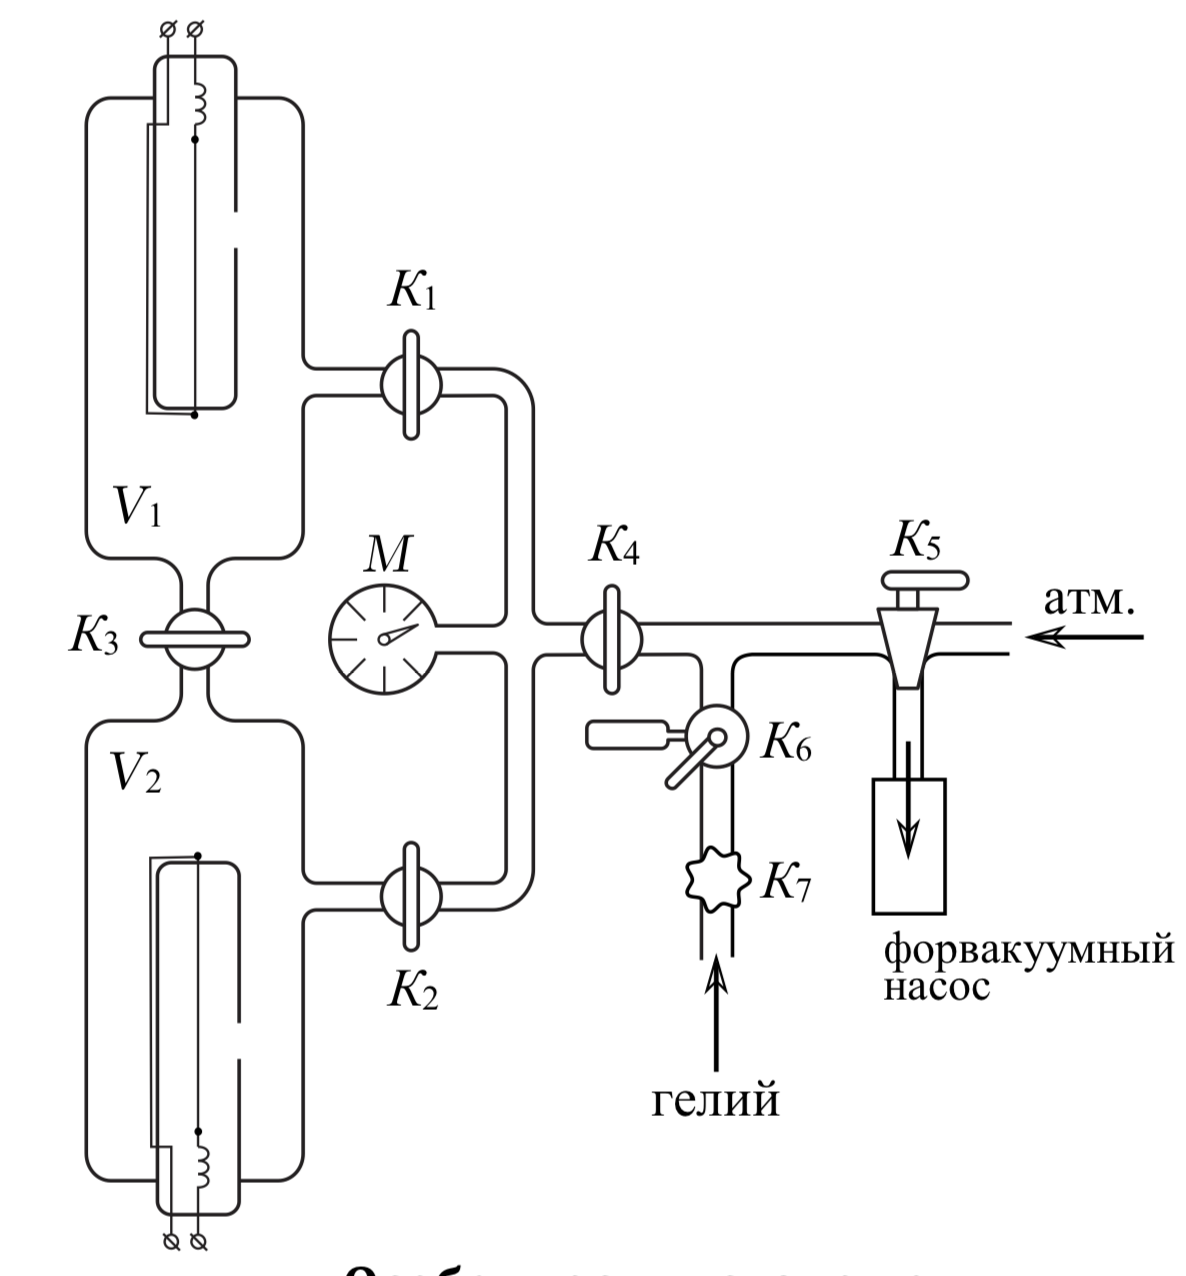
\includegraphics[scale=0.4]{scheme.png}
\label{scheme}
\caption{Схема установки}
\end{figure}
Общая схема установки представлена на рис.\ref{scheme}.
Установка состоит из форвакуумного баллона (ФБ), высоковакуумного диффузионного насоса (ВН), высоковакуумного баллона (ВБ), масляного (М) и ионизационного (И) манометров, термопарных манометров ($M_1 \textit{и} \hspace{1mm} M_2$), форвакуумного насоса (ФН) и соединительных кранов $K_1, ..., K_6$.
\subsection{Насосы}
\subsubsection{Форвакуумный насос}
Устройство и принцип действия ротационного пластинчатого форвакуумного насоса схематически представлены на рис. \ref{pump}.
\begin{figure}[!h]
\centering
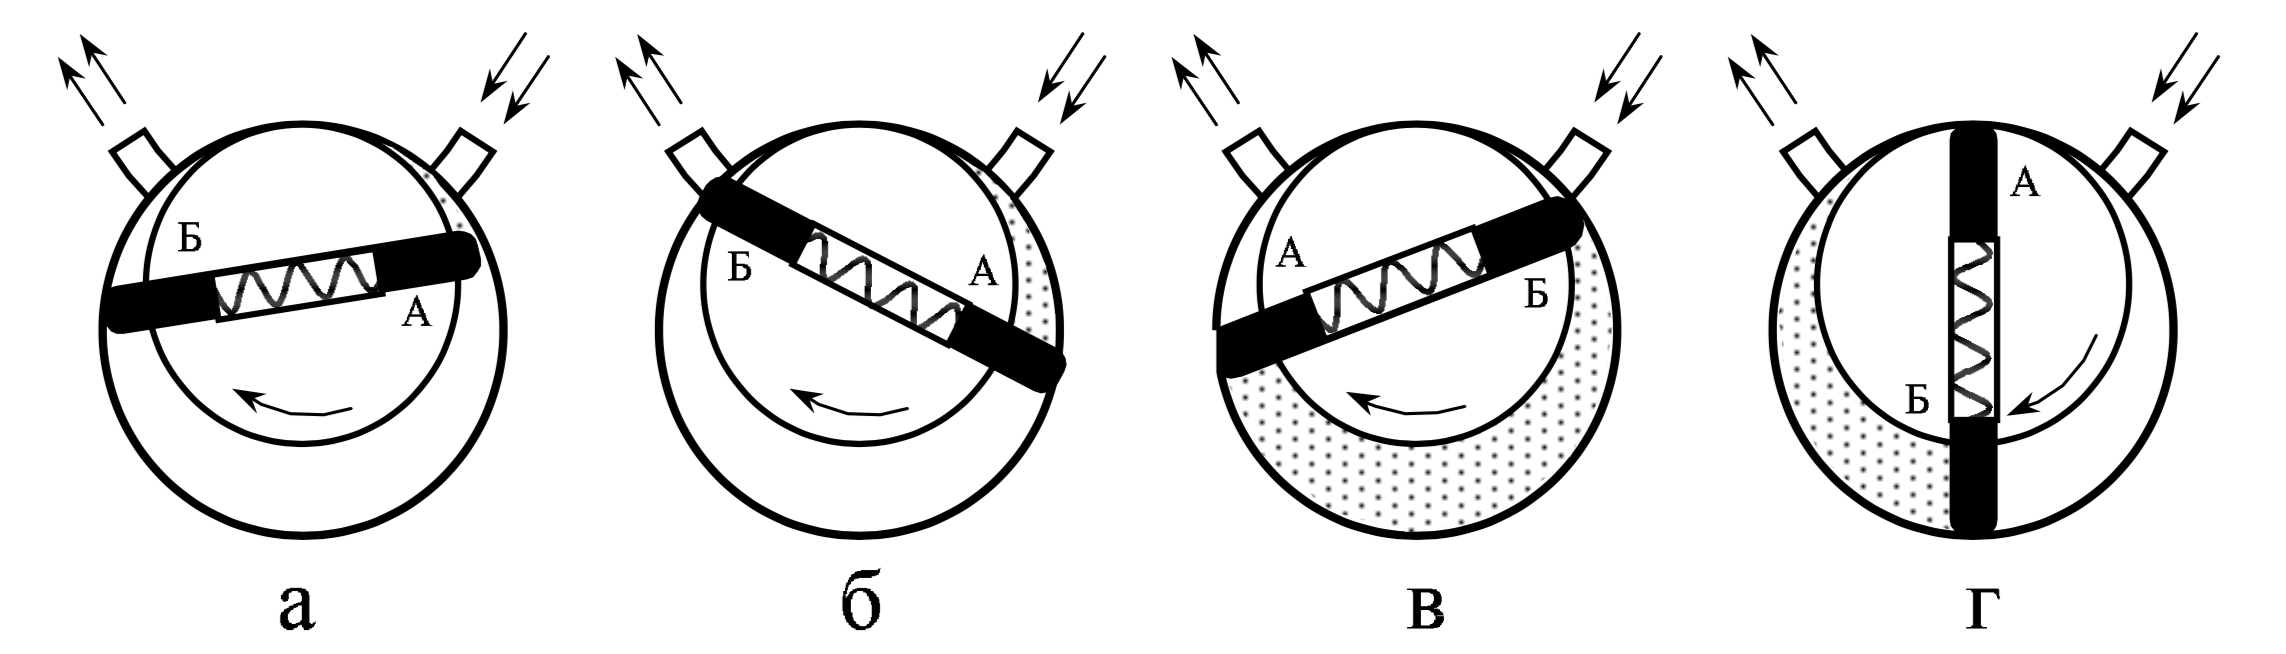
\includegraphics[scale=0.4]{pump1.png}
\label{pump1}
\caption{Принцип работы форвакуумного насоса}
\end{figure}
В цилиндрической полости массивного корпуса размещен эксцентрично ротор, постоянно соприкасающийся своей верхней частью с корпусом. В диаметральный разрез ротора вставлены две пластины, раздвигаемые пружиной и плотно прижимаемые к поверхности полости. Они разделяют объем между ротором и корпусом на две части.
При работе насоса происходят циклические изменения объема воздуха, поступаемые из откачиваемого объема. На рис \ref{pump1} в положениях а и б пластина А засасывает разреженный воздух из откачанного объема, а пластина Б вытесняет ранее захваченный воздух в атмосферу. В положениях в и г просисходит то же самое, только пластины меняются ролями.
\subsubsection{Диффузионный насос}
Принцип работы диффузионного насоса основывается на диффузии молекул разреженного газа в пары масла. Попавшие в струю паров молекулы увлекаются ею и уже не возвращаются. Таким образом происходит повышение разреженности воздуха.
\begin{figure}[!h]
\centering
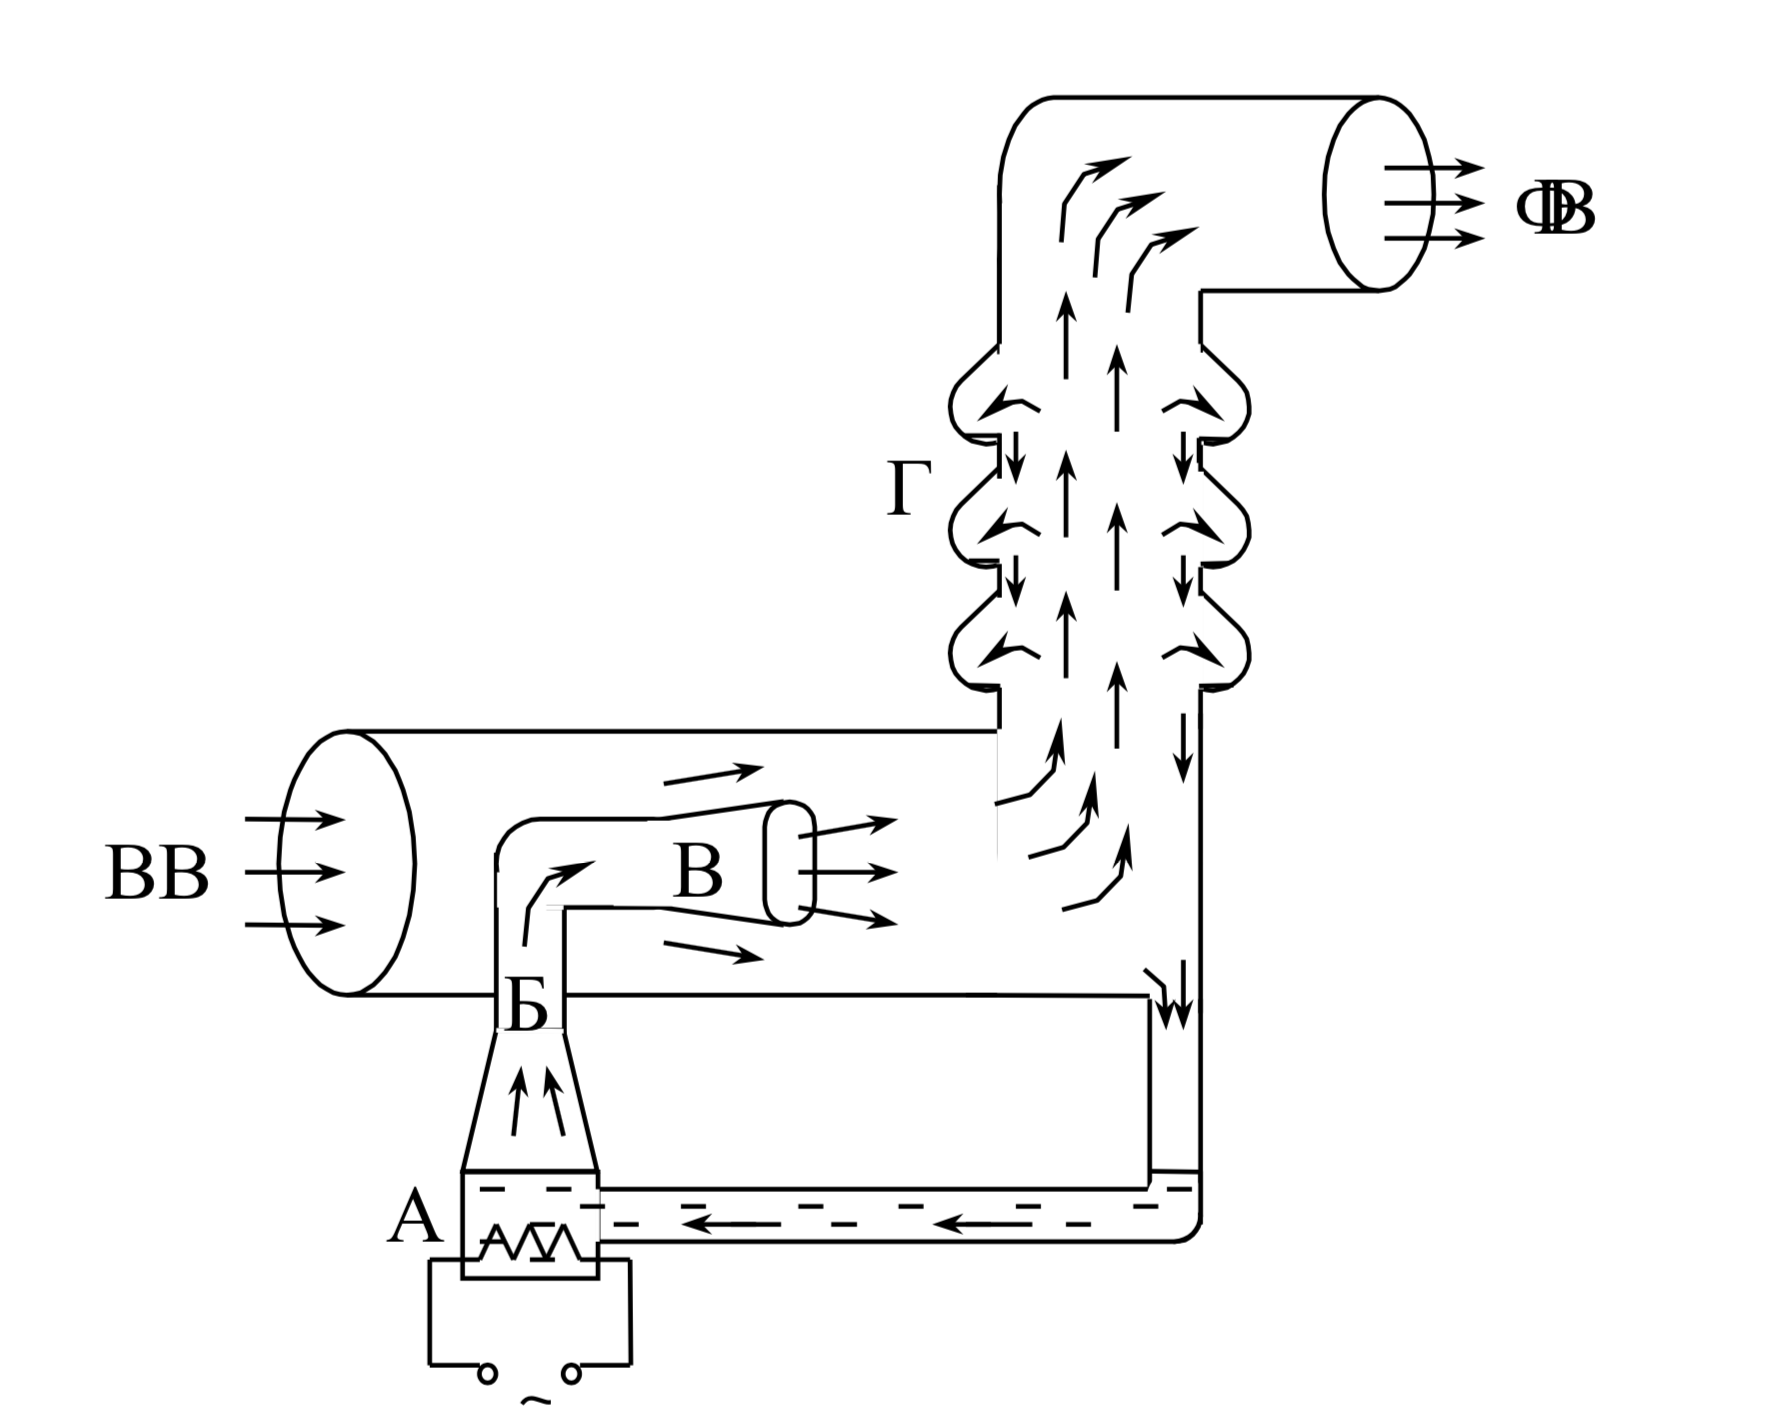
\includegraphics[scale=0.4]{pump2.png}
\label{pump_2}
\caption{Устройство диффузионного насоса}
\end{figure}
Устройство диффузионного насоса схематически показано на рис. \ref{pump_2}. Масло, налитое в сосуд А, подогревается электрической печкой. Пары масла поднимаются по трубе Б и вырываются из сопла В, увлекая за собой молекулы воздуха. Далее струя попадает в вертикальную трубу Г, где масло конденсируется и стекает вниз, а молекулы воздуха откачиваются форвакуумным насосом. Даление насыщенных паров масла много больше $5 \cdot 10^{-2}$ торр, поэтому пары масла создают мощную струю.]
\subsection{Манометры}
\subsubsection{Масляный манометр}
Масляный манометр представляют собой U-образную трубку, до половины наполненную вязким маслом, имеющим низкое давление насыщенных паров. Из-за малой плотности масла ($\rho = 0,9 \textit{г/см$^3$}$) можно измерять только небольшие разности давлений (до нескольких торр). 
\subsubsection{Термопарный манометр}
Чувствительным элементом манометра является платино-платинорадиевая термопара, спаянная с никелевой нитью накала и заключенная в стеклянный баллон. Устройство термопары пояснено на рис. \ref{termopare}. По нити накала НН пропускается ток постоянной величины. Для установки тока служит потенциометр R. Термопара ТТ присоединяется к милливольтметру, показания которого определяются температурой нити накала и зависят от отдачи тепла в окружающее пространство. 

При улучшении вакуума средний свободный пробег молекул становится сравнимыми с диметром нити, теплопровод падает и возрастает температура нити. При вакууме $\sim 10^{-3}$ торр температура нити становится практически постоянной.

Для оценки вакуума с помощью термопарного манометра используют градуировочную кривую(см рис.\ref{curve}).
 \begin{figure}[H]
\begin{floatrow}
\ffigbox{\caption{Устройство термопарного манометра}\label{lamp}}%
 {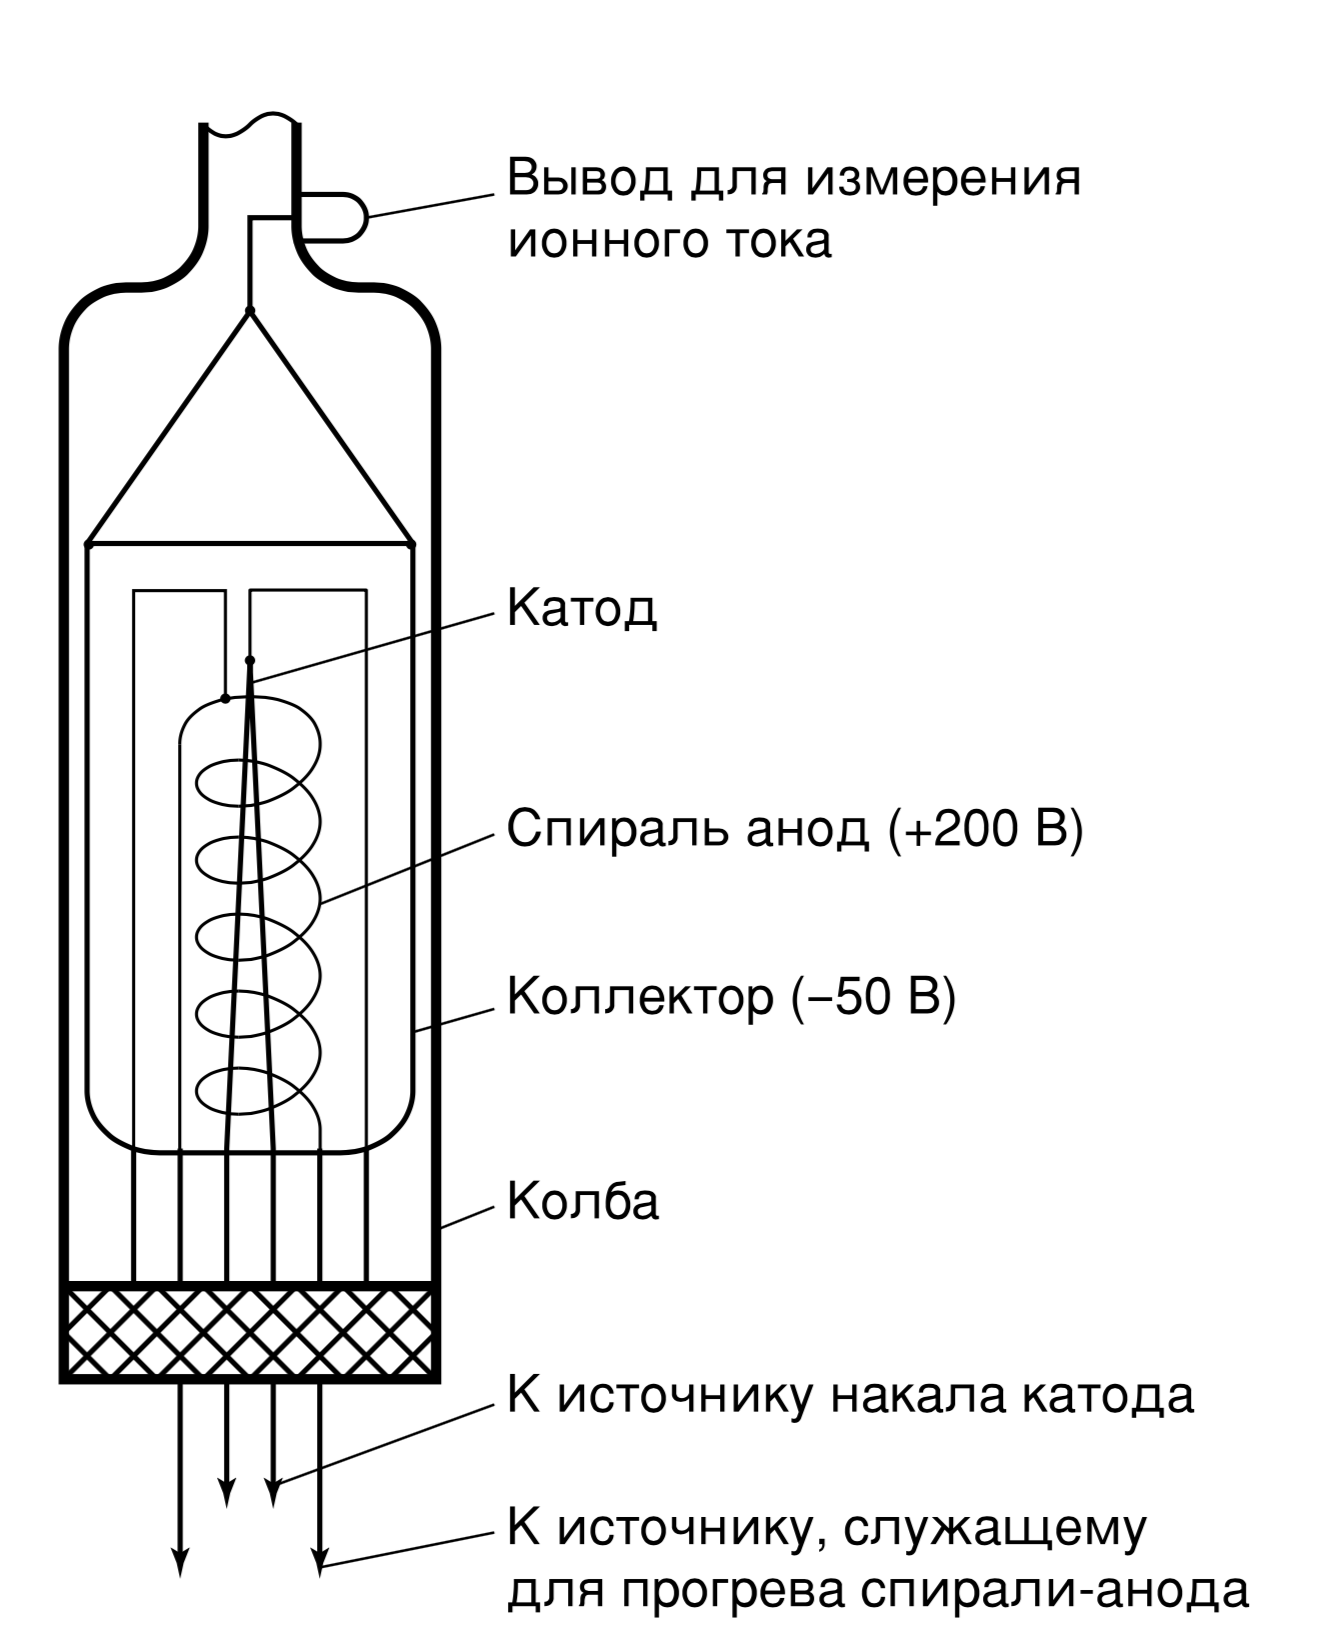
\includegraphics[scale=0.3]{lamp.png}}
\ffigbox{\caption{Градуировочная кривая}\label{curve}}%
{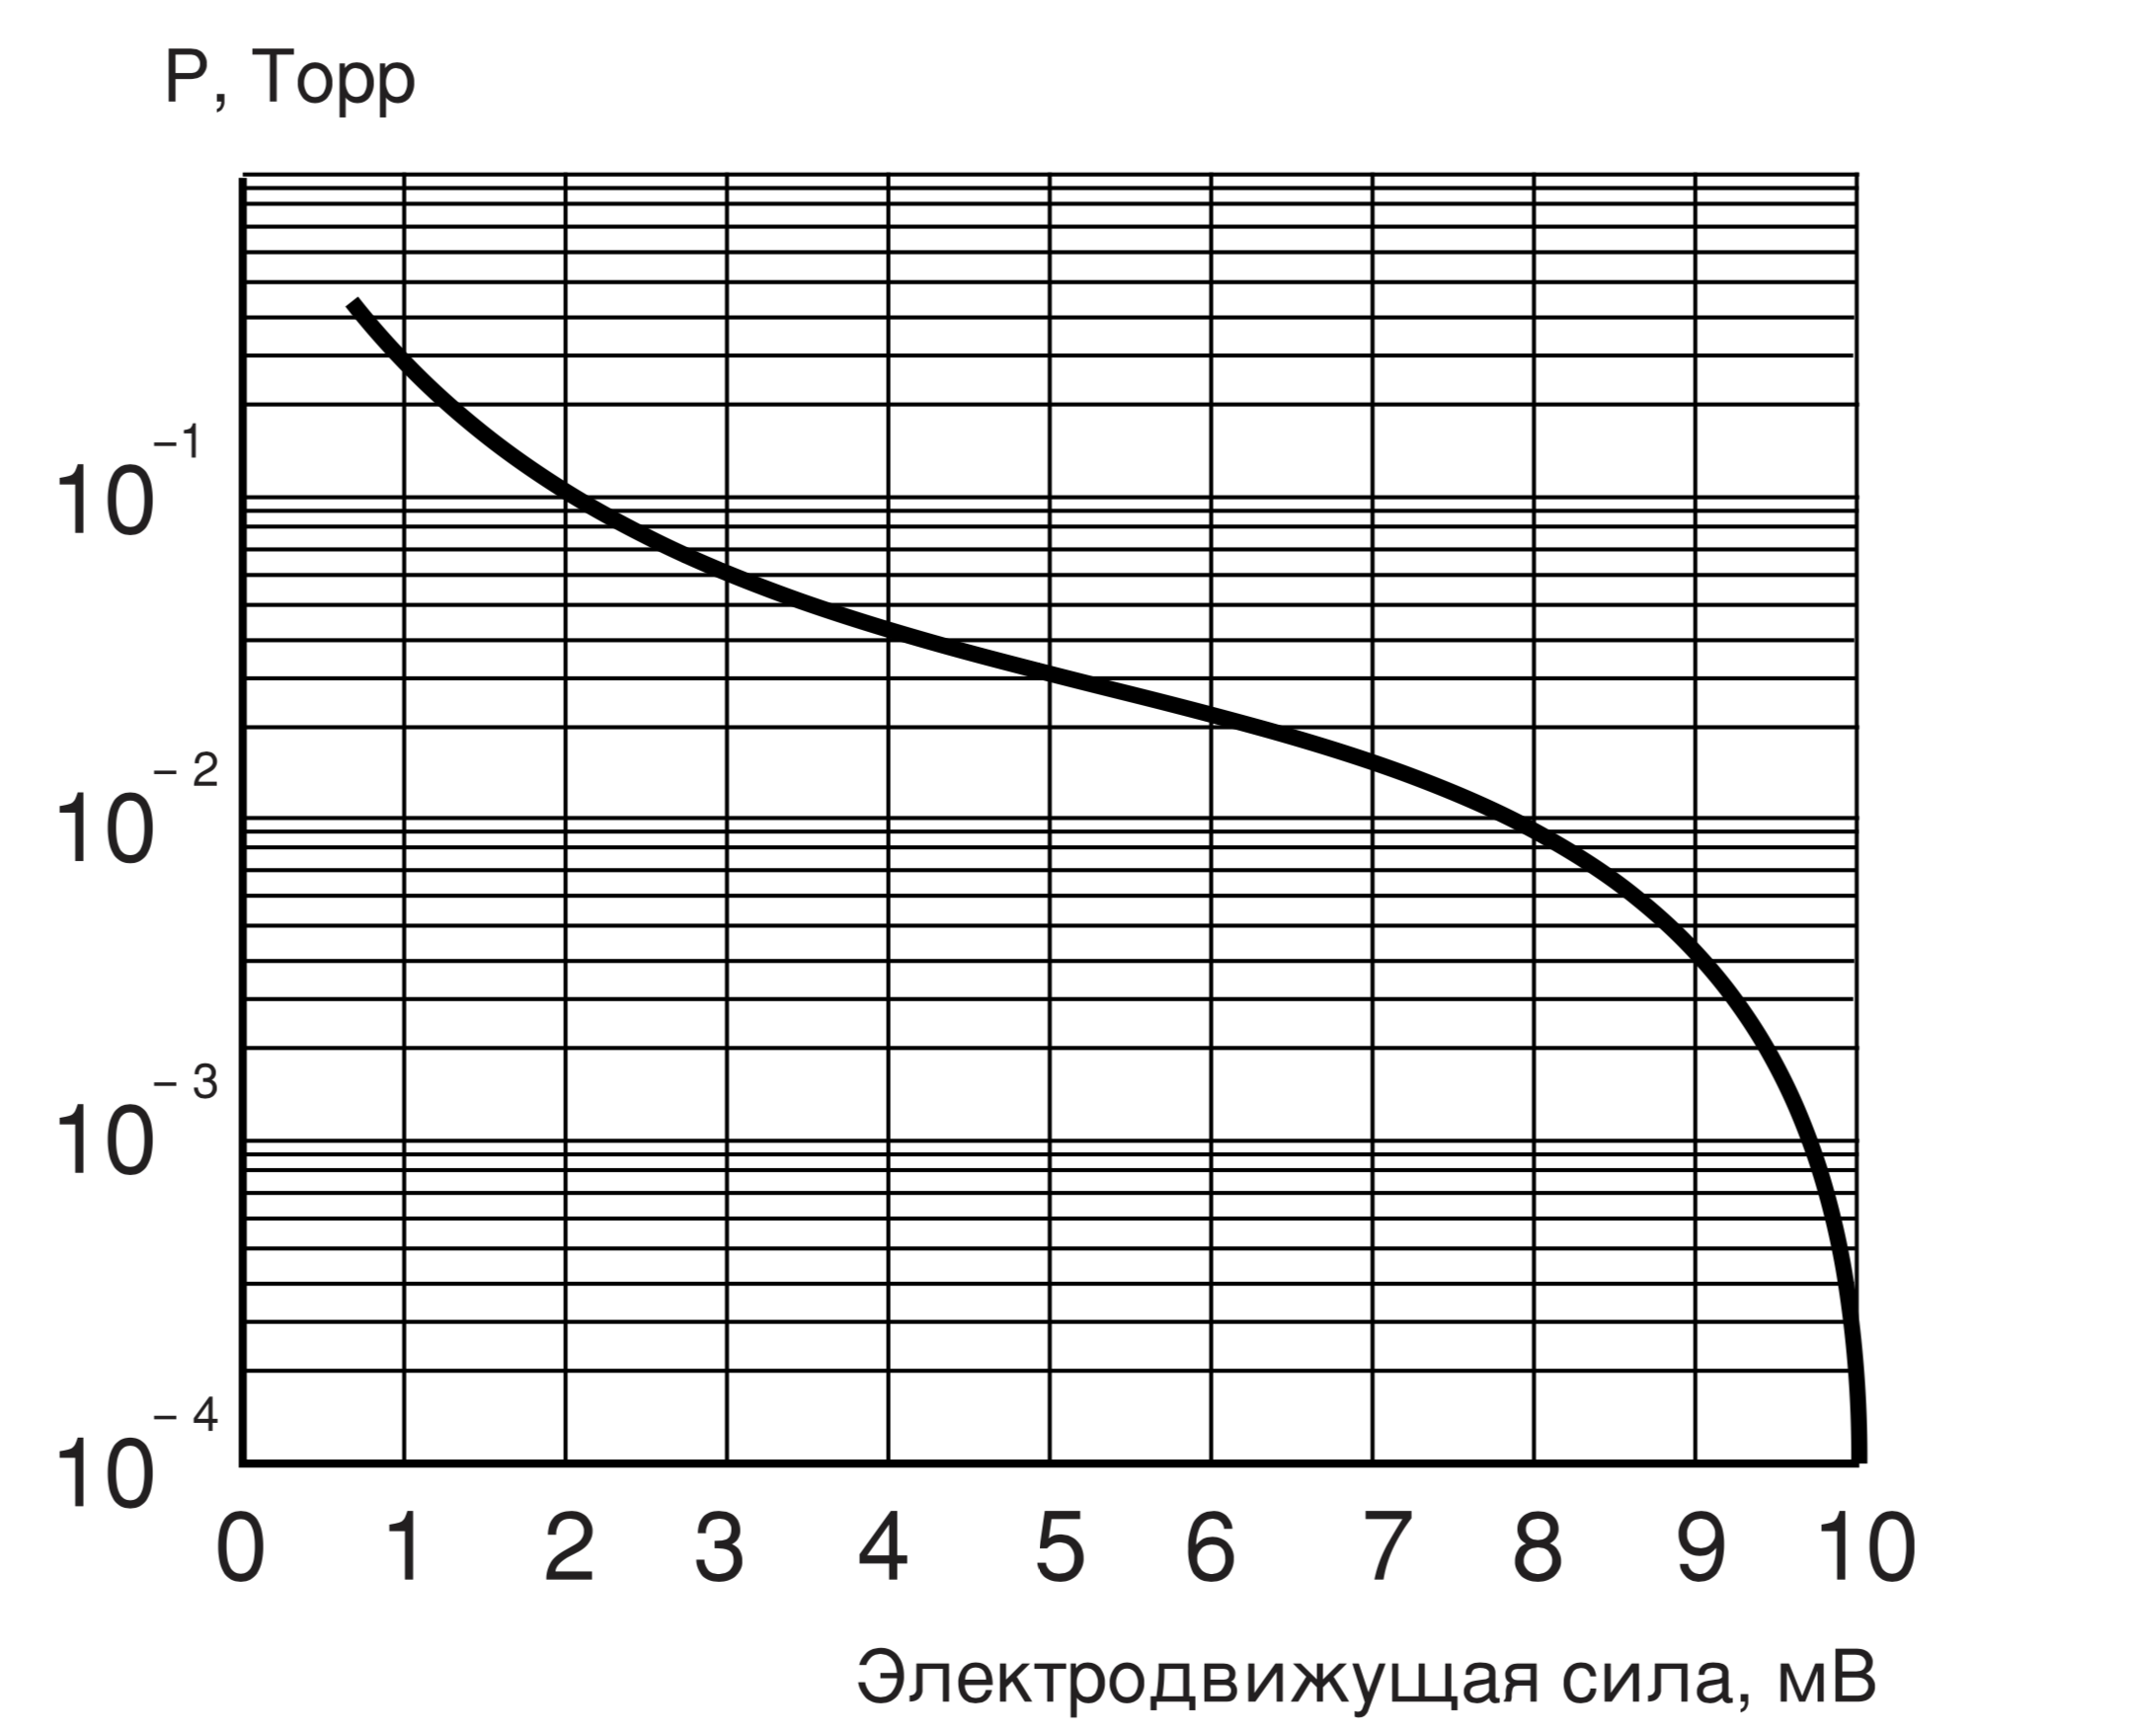
\includegraphics[scale=0.25]{curve.png}}         
\end{floatrow}
\end{figure}
\subsubsection{Ионизационный манометр}
Схема ионизационного манометра представлена на рис. \ref{lamp1}. 

\begin{wrapfigure}{r}{0.2\linewidth}\label{lamp1}
	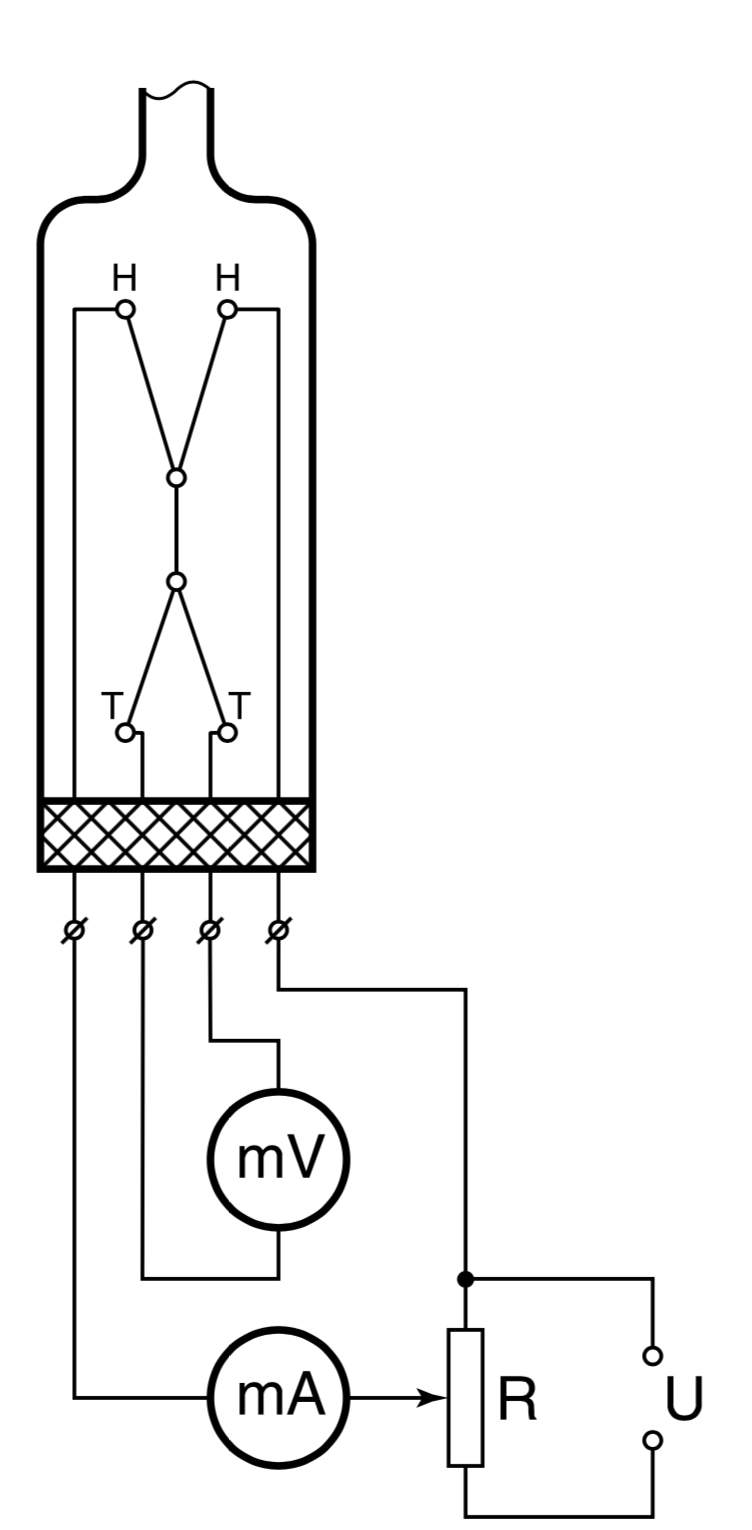
\includegraphics[width=\linewidth]{lamp1.png}
	\caption{Схема ионизационного манометра}
\end{wrapfigure}
Он представляет собой трехэлектродную лампу. Электроны испускаются нагретым катодом и увлекаются электрическим полем к аноду, имеющему форму спирали. Под влиянием поля коллектора электроны многократно пересекают пространство между катодом и коллектором и ионизируют молекулы газа. Образовавшиеся ионы притягиваются к коллектору и определяют  его ток. Лампа перегорает при  давлениии свыше $10^{-3}$ торр, поэтому необходимо производить измерения при давлениях, не превышающих данного значения.
\subsection{Откачка воздуха}
Производительность насоса определяются \textit{скоростью откачки $W$} -- объемом газа, удаляемым из сосуда при данном давлении за единицу времени.  Определим предельное давление, достижимое при откачке воздуха:
\begin{equation}
-VdP = (PW - Q_\textit{д} -  Q_\textit{н} -  Q_\textit{и})dt,
\end{equation}
где $Q_\textit{д}$ -- количество газа, десорбирующегося с поверхности откачиваемого объема в единицу времени, $Q_\textit{н}$ -- поток газа, поступающего из насоса обратно в систему, $Q_\textit{и}$ -- количество газа, проникающего в систему извне в единицу времени. 

При  $P = P_\textit{пр} \hspace{0.8cm} \dfrac{dP}{dt} = 0$, поэтому
\begin{equation}
P_\textit{пр}W = Q_\textit{д} +  Q_\textit{н} +  Q_\textit{и}
\end{equation}
Полагая, что все $Q$ постоянны, интегрируя (1) и применяя (2), получаем
\begin{equation}
P = P_0 \exp \left(-\frac{W}{V}t\right) + P_{\textit{пр}}.
\end{equation}
Постоянная меры откачки $\tau = V/W$ является мерой эффективности откачной системы.
\section{Выполнение работы:}
\subsection{Определение объема форвакуумной и высоковакуумной частей установки}
\begin{enumerate}
\item
Определим объемы сосудов. Для этого закроем краны $K_5$ и $K_6$ (при этом в капиллярах <<запирается>> объем $V = 50$ см$^3$ ), затем закроем краны $K_1$ и $K_2$, подключив установку к форвакуумному насосу, и кран $K_3$, изолируя таким образом высоковакуумную часть от форвакуумной. Включим форвакуумный насос и откачаем установку. Измерим полученное давление масляным манометром.
\item
Затем откроем кран $K_5$. При этом <<запертый>> воздух заполнит всю форвакуумную часть установки. Измерим изменение давления манометром: \\
$h_1 = 16,5$ см \\
$h_2 = 31,2$ см \\
$\Delta h_\textit{фв} = h_2 - h_1 = 14,7$ см \\
$P = \rho g \Delta h = 1274,9$ Па

Из закона Бойля-Мариотта получим, что объем форвакуумной части установки $V_\textit{фв} = \dfrac{P_0V_0}{P}$. Отсюда можно получить значение $V_\textit{фв} = 3972,7$ см$^3$.
\item
Откроем кран К3, соединяя форвакуумную и высоковакуумную часть. Измерим изменение давления масляным манометром. Рассуждая аналогично, получим значение объема высоковакуумной части $V_\textit{вв}$. \\
$h_1 = 18$ см \\
$h_2 = 29,8$ см \\
$\Delta h_\textit{полн} = h_2 - h_1 = 11,8$ см \\
$P = \rho g \Delta h = 1274,9$ Па \\
$V_\textit{полн} = 4949,1$ см$^3$ \\
$V_\textit{вв} = V_\textit{полн} - V_\textit{фв} = 976,4$ см$^3$
\item
Погрешность измерений: \\
\[\sigma_V = \sqrt{(\dfrac{\sigma_{V_0}}{V_0})^2 + (\dfrac{\sigma_{\Delta h}}{\Delta h})^2 }\]
Отсюда $V_\textit{фв} = (3972,7 \pm 239,9)$ см$^3$, $V_\textit{вв} = (976,4 \pm 59,1)$ см$^3$

\end{enumerate}
\subsection{Получение высокого вакуума и измерение скорости откачки}
\begin{enumerate}
\item
Откачаем установку форвакуумным насосом и, когда даление станет достаточно низким $< 3\cdot 10^{-2}$ торр, начнем высоковакуумную откачку. Дождемся, пока давление в системе упадет до предельного значения.
\item
Проведем измерение значения предельного давления с помощью ионизационного манометра: \\
$P_\textit{пр} = 6,3 \cdot 10^{-5}$ торр
\item
Найдем скорость откачки по улучшению вакуума во время откачки. Для этого откроем кран $K_3$ и измерим изменение давления в зависимости от времени. Запишем результаты в таблицу 1.
\begin{table}[!h]
\centering
\begin{tabular}{|l|c|c|}
\toprule
 t, c & $P, 10^{-4}$ торр & $\ln (P - P_\textit{пр})$  \\
\midrule
0   &   6,4 &   1,76 \\
1   &   5,6 &   1,61 \\
2   &   4,2 &   1,28 \\
3   &   3,4 &   1,03 \\
4   &   2,8 &   0,79 \\
5   &   2,3 &   0,53 \\
6   &   1,9 &   0,26 \\
7   &   1,6 &   0,00 \\
8   &   1,4 &   -0,22 \\
9   &   1,2 &   -0,51 \\
10  &   1,1 &   -0,69 \\
11  &   0,9 &   -1,20 \\
12  &   0,8 &   -1,61 \\
\bottomrule
\end{tabular}
\caption{Измерения при улучшении вакуума}
\end{table}
\item
По полученным данным построим график зависимости  $\ln (P - P_\textit{пр}) $ от t:
\begin{figure}[!h]
\centering
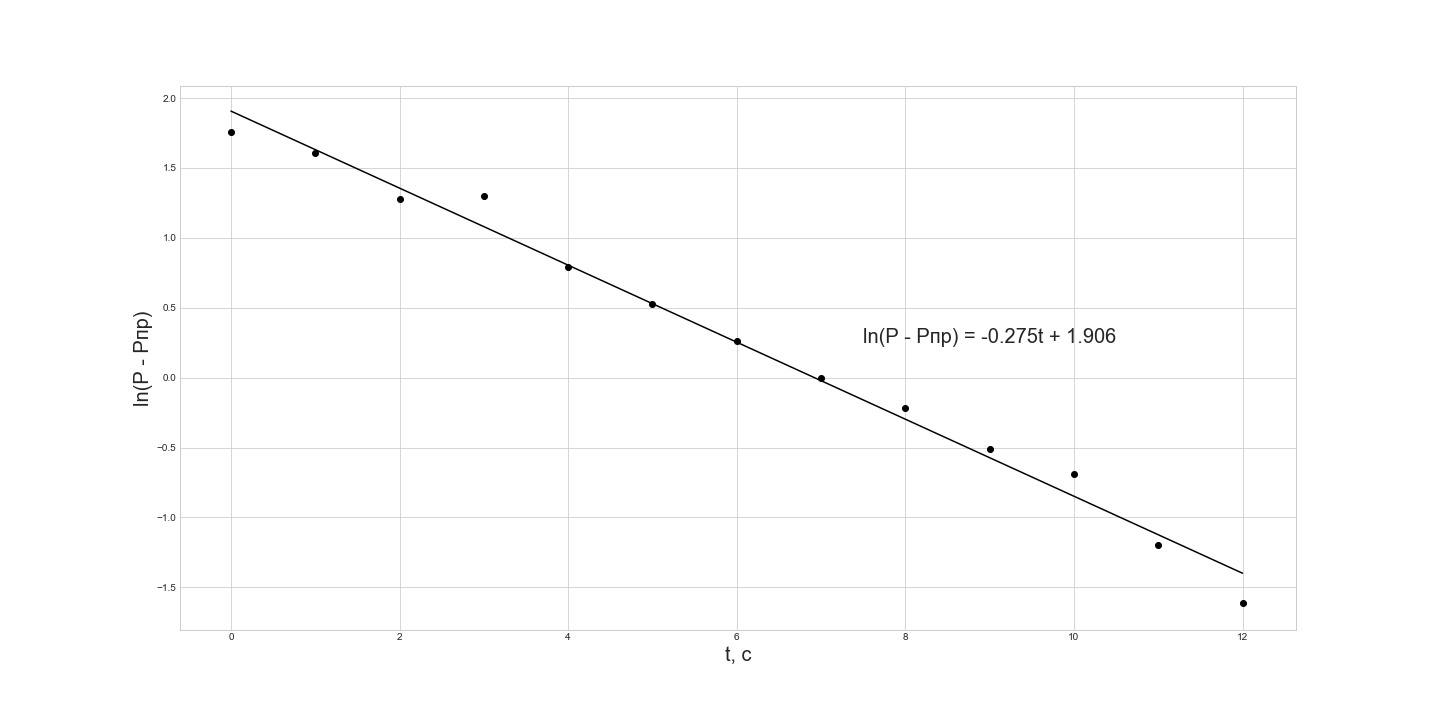
\includegraphics[scale=0.4]{graph.png} 
\caption{Улучшение вакуума}
\end{figure}
\[\dfrac{1}{\tau} = -\dfrac{W}{V_\textit{вв}} = -0,275\]
\[W = 0,275 \cdot 0,976 \approx 0,268 \textit{л/с}\]
\[ \varepsilon_W = \sqrt{ (\varepsilon_\tau)^2 + (\varepsilon_V)^2} \approx 7\% \]
Таким образом $W = 0,268 \pm 0,019 \textit{л/с}$ \\
Оценим величину потока $Q_\textit{н}$ (в Н$\cdot$м/с):
\[V_\textit{вв}dP = (Q_\textit{д} + Q_\textit{н})dt\]
\[Q_\textit{н} = PW \approx 1,1 \cdot 10^{-5}\]
\item
Откроем кран $K_6$, введя таким образом искусственную течь в установку. Измерим установившееся давление: \\
$P_\textit{уст} = 1,5 \cdot 10^{-4}$ торр \\
Количество газа, протекающего через капилляр: $\dfrac{d(PV)}{dt} = \dfrac{4}{3}r^3\sqrt{\dfrac{2\pi RT}{\mu}}\dfrac{P_\textit{фв} - P_\textit{уст}}{l}$  \\
$P_\textit{уст}W = P_\textit{пр}W + \frac{d}{dt}(PV)_\textit{капилл} \rightarrow W = \dfrac{4}{3l}r^3\sqrt{\dfrac{2\pi RT}{\mu}}\dfrac{P_\textit{фв} - P_\textit{уст}}{P_\textit{уст} - P_\textit{пр}} \approx 6,98\cdot 10^{-5}$ м$^3$/с = 6,98 $\cdot 10^{-2}$ л/с \\
$\varepsilon_W = \sqrt{\varepsilon_P^2 + \varepsilon_r^2 + \varepsilon_l^2} \approx 13 \%$
\end{enumerate}
Полученное значение $W = (6,98 \pm 0,91)  \cdot 10^{-2}$ л/с 
\section{Вывод:}
При улучшении вакуума при откачке полученное значение скорости откачки равно $W = (0,268 \pm 0,019)$ л/с, а при введении искусственной течи  $W = (6,98 \pm 0,91)  \cdot 10^{-2}$ л/с. Расхождения в значениях вызваны погрешностями и недостаточной точностью измерительных приборов, а также утечкой воздуха из установки.
\end{document}
